\qrchapter{https://forgottenpillar.com/rsc/en-fp-chapter1}{The historical context}


\qrchapter{https://forgottenpillar.com/rsc/en-fp-chapter1}{Le contexte historique}


Ellen White recalled encountering the same sentiments in \textit{The Living Temple} that she had warned against early in her ministry:


Ellen White se souvenait d'avoir rencontré le même raisonnement dans \textit{Le Temple Vivant} contre lequel elle avait mis en garde au début de son ministère :


\egw{As we read \normaltext{[The Living Temple]}, I recognized the very sentiments against which I had been bidden to speak in warning \textbf{during the early days of my public labors}. \textbf{When I first left \underline{the State of Maine, it was to go through Vermont and Massachusetts}}, to bear a testimony \textbf{against these sentiments}. ‘Living Temple’ contains the alpha of these theories. I knew that the omega would follow in a little while; and I trembled for our people. I knew that I must warn our brethren and sisters \textbf{not to enter into controversy over \underline{the presence and personality of God}}. The statements made in ‘Living Temple’ in regard to this point are incorrect. The scripture used to substantiate the doctrine there set forth, is scripture misapplied.}[SpTB02 53.2; 1904][https://egwwritings.org/read?panels=p417.271]


\egw{En lisant \normaltext{[Le Temple Vivant]}, j'ai reconnu les mêmes raisonnements contre lesquels j'avais été chargée de mettre en garde \textbf{pendant les premiers jours de mon ministère public}. \textbf{Lorsque j'ai quitté pour la première fois \underline{l'État du Maine, c'était pour traverser le Vermont et le Massachusetts}}, pour rendre témoignage \textbf{contre ces raisonnements}. ‘Le Temple Vivant’ contient l'alpha de ces théories. Je savais que l'oméga suivrait peu après ; et je tremblais pour notre peuple. Je savais que je devais avertir nos frères et sœurs \textbf{de ne pas entrer dans une controverse sur \underline{la présence et la personnalité de Dieu}}. Les déclarations faites dans ‘Le Temple Vivant’ à ce sujet sont incorrectes. L'Écriture utilisée pour étayer la doctrine qui y est exposée est une Écriture mal appliquée.}[SpTB02 53.2; 1904][https://egwwritings.org/read?panels=p417.271]


She pinpointed her first encounter with these views: \egwinline{When I first left \textbf{the State of Maine}, it was to go through Vermont and Massachusetts, \textbf{to bear a testimony against these sentiments.}} Her biography, written by her grandson Arthur Lacey White, provides further context on these sentiments. In \textit{Ellen White: The Early Years}, under the section \textit{Wrestling with the Views of the Spiritualizers}, her experiences in eastern Maine reveal more about the controversy over the personality of God and its implications.


Elle a précisé sa première rencontre avec ces points de vue : \egwinline{Lorsque j'ai quitté pour la première fois \textbf{l'État du Maine}, c'était pour traverser le Vermont et le Massachusetts, \textbf{pour rendre témoignage contre ces raisonnements.}} Sa biographie, écrite par son petit-fils Arthur Lacey White, fournit plus de contexte sur ces raisonnements. Dans \textit{Ellen White: Les Premières Années}, sous la section \textit{Lutter contre les vues des spiritualistes}, ses expériences dans l'est du Maine révèlent davantage sur la controverse concernant la personnalité de Dieu et ses implications.


\othersQuote{\textbf{\underline{In eastern Maine} Ellen was traveling} and working \textbf{in the atmosphere of the spiritualizers who had \underline{allegorized away heaven, God, Jesus, and the Advent hope}}. In the vision at Exeter in mid-February she seemed to be \textbf{in the presence of Jesus, and she was eager to procure answers to some \underline{vital questions}}.}[ALW, 1BIO 79.4; 1985][https://egwwritings.org/read?panels=p668.582]


\othersQuote{\textbf{\underline{Dans l'est du Maine}, Ellen voyageait} et travaillait \textbf{dans l'atmosphère des spiritualistes qui avaient \underline{allégorisé le ciel, Dieu, Jésus et l'espérance de l'Avènement}}. Dans la vision à Exeter à la mi-février, elle semblait être \textbf{en présence de Jésus, et elle était impatiente d'obtenir des réponses à certaines \underline{questions vitales}}.}[ALW, 1BIO 79.4; 1985][https://egwwritings.org/read?panels=p668.582]


\othersQuoteNoGap{I asked Jesus if \textbf{His Father had a form like Himself}. \textbf{He said He had}, but I could not behold it, for said He, ‘If you should once behold the glory of \textbf{His person}, you would cease to exist.’—Early Writings, 54.}[ALW, 1BIO 79.5; 1985][https://egwwritings.org/read?panels=p668.583]


\othersQuoteNoGap{J'ai demandé à Jésus si \textbf{Son Père avait une forme comme Lui-même}. \textbf{Il a dit qu'Il en avait une}, mais je ne pouvais pas la contempler, car, dit-Il, ‘Si tu devais contempler une seule fois la gloire de \textbf{Sa personne}, tu cesserais d'exister.’ — Premiers Écrits, 54.}[ALW, 1BIO 79.5; 1985][https://egwwritings.org/read?panels=p668.583]


\othersQuoteNoGap{This was not the only occasion Ellen was to converse with Jesus and the angel \textbf{about the \underline{person of Jesus} and concerning \underline{God being a personal being}}. \textbf{\underline{The answers satisfied her fully that the spiritualizers were in gross error}}.}[ALW, 1BIO 80.1; 1985][https://egwwritings.org/read?panels=p668.586]


\othersQuoteNoGap{Ce n'était pas la seule occasion où Ellen devait converser avec Jésus et l'ange \textbf{au sujet de la \underline{personne de Jésus} et concernant le fait que \underline{Dieu est un être personnel}}. \textbf{\underline{Les réponses l'ont pleinement satisfaite que les spiritualistes étaient dans une grave erreur}}.}[ALW, 1BIO 80.1; 1985][https://egwwritings.org/read?panels=p668.586]


The vision Arthur Lacey White referred to is known as the \textit{vision on the personality of God}, which we will examine later. This vision confirms that the doctrine of the \emcap{personality of God} teaches that God the Father has a form, just as Jesus does. It specifically addresses the \others{\textbf{person of Jesus} and concerning \textbf{God being a personal being}.}


La vision à laquelle Arthur Lacey White a fait référence est connue comme la \textit{vision sur la personnalité de Dieu}, que nous examinerons plus tard. Cette vision confirme que la doctrine de la \emcap{personnalité de Dieu} enseigne que Dieu le Père a une forme, tout comme Jésus. Elle aborde spécifiquement la \others{\textbf{personne de Jésus} et concernant le fait que \textbf{Dieu est un être personnel}.}


\begin{figure}[t]
    \centering
    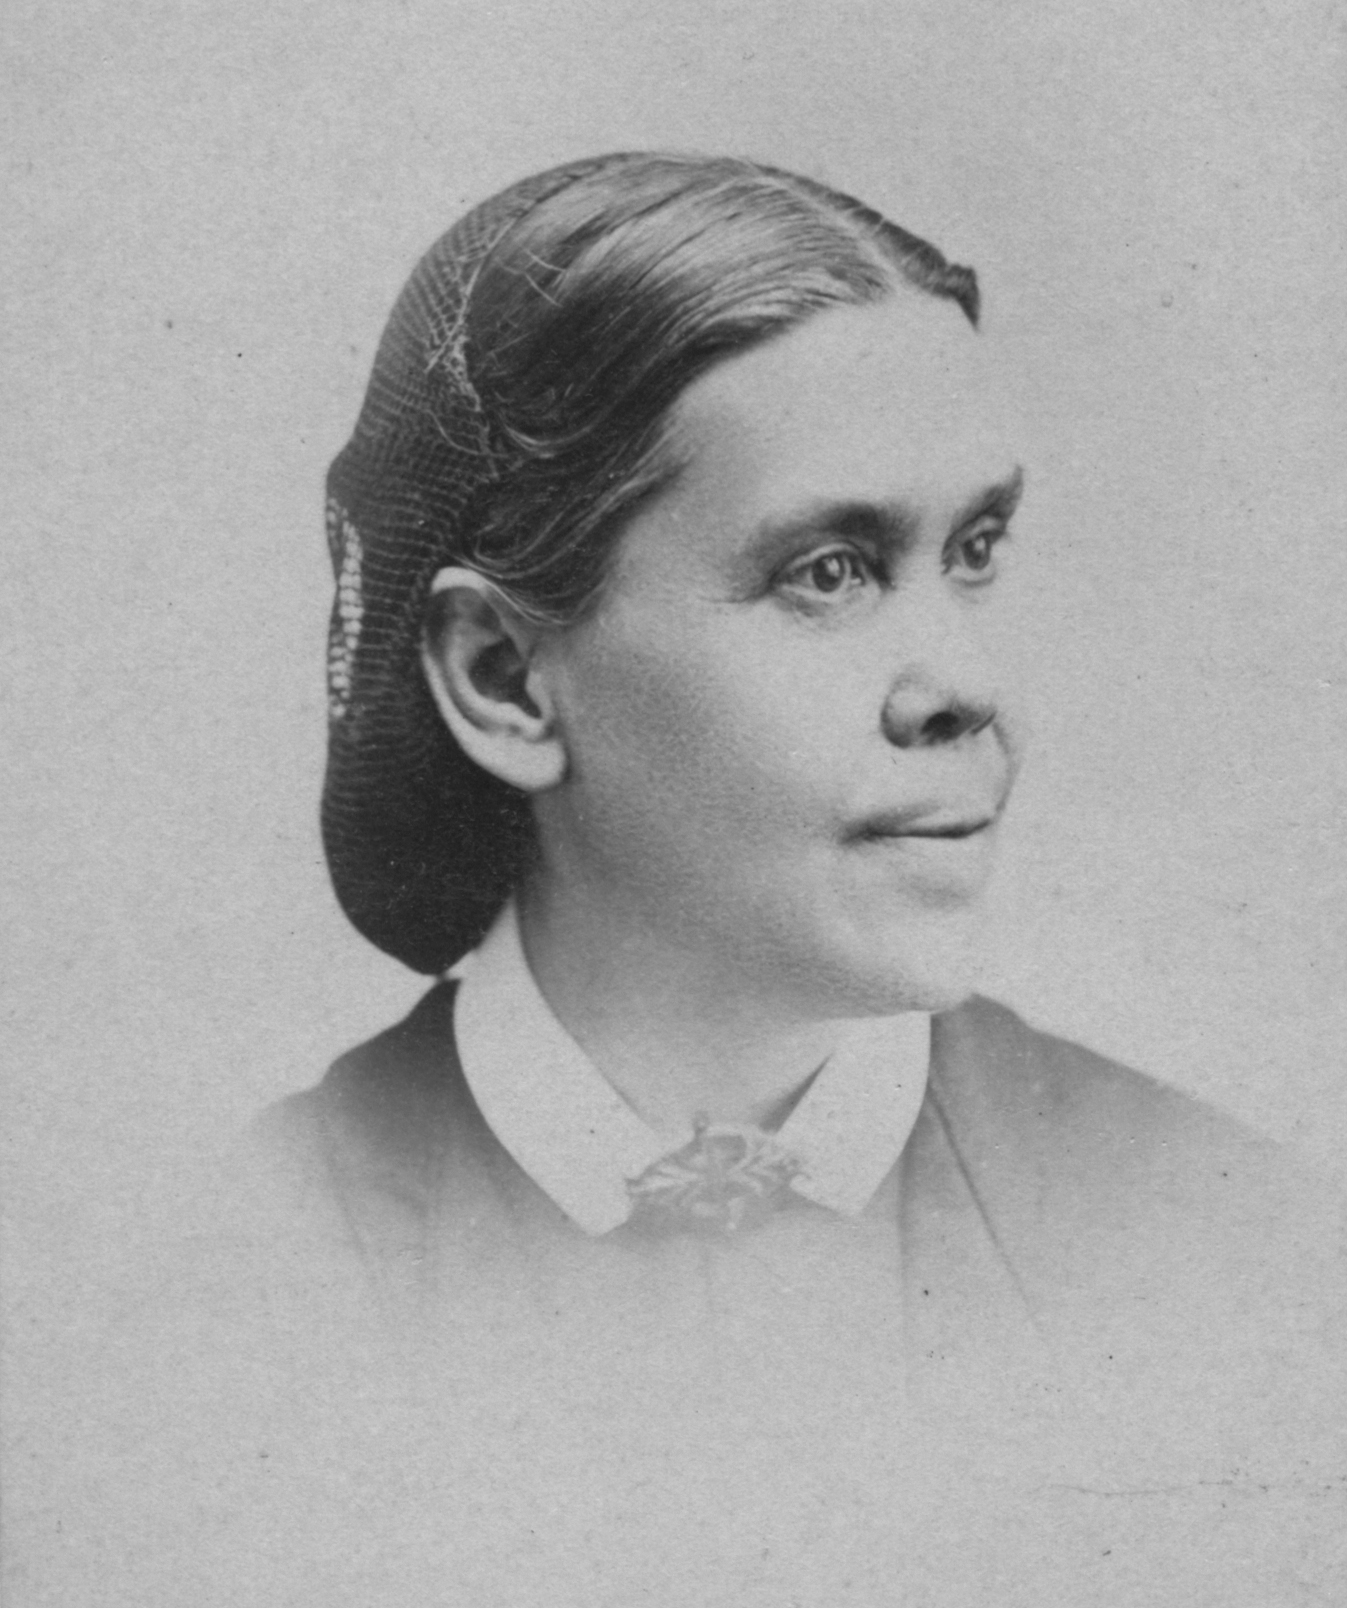
\includegraphics[width=0.65\linewidth]{images/ellen-white.jpg}
    \caption*{Ellen G. White}
    \label{fig:ellen-g-white}
\end{figure}


\begin{figure}[t]
    \centering
    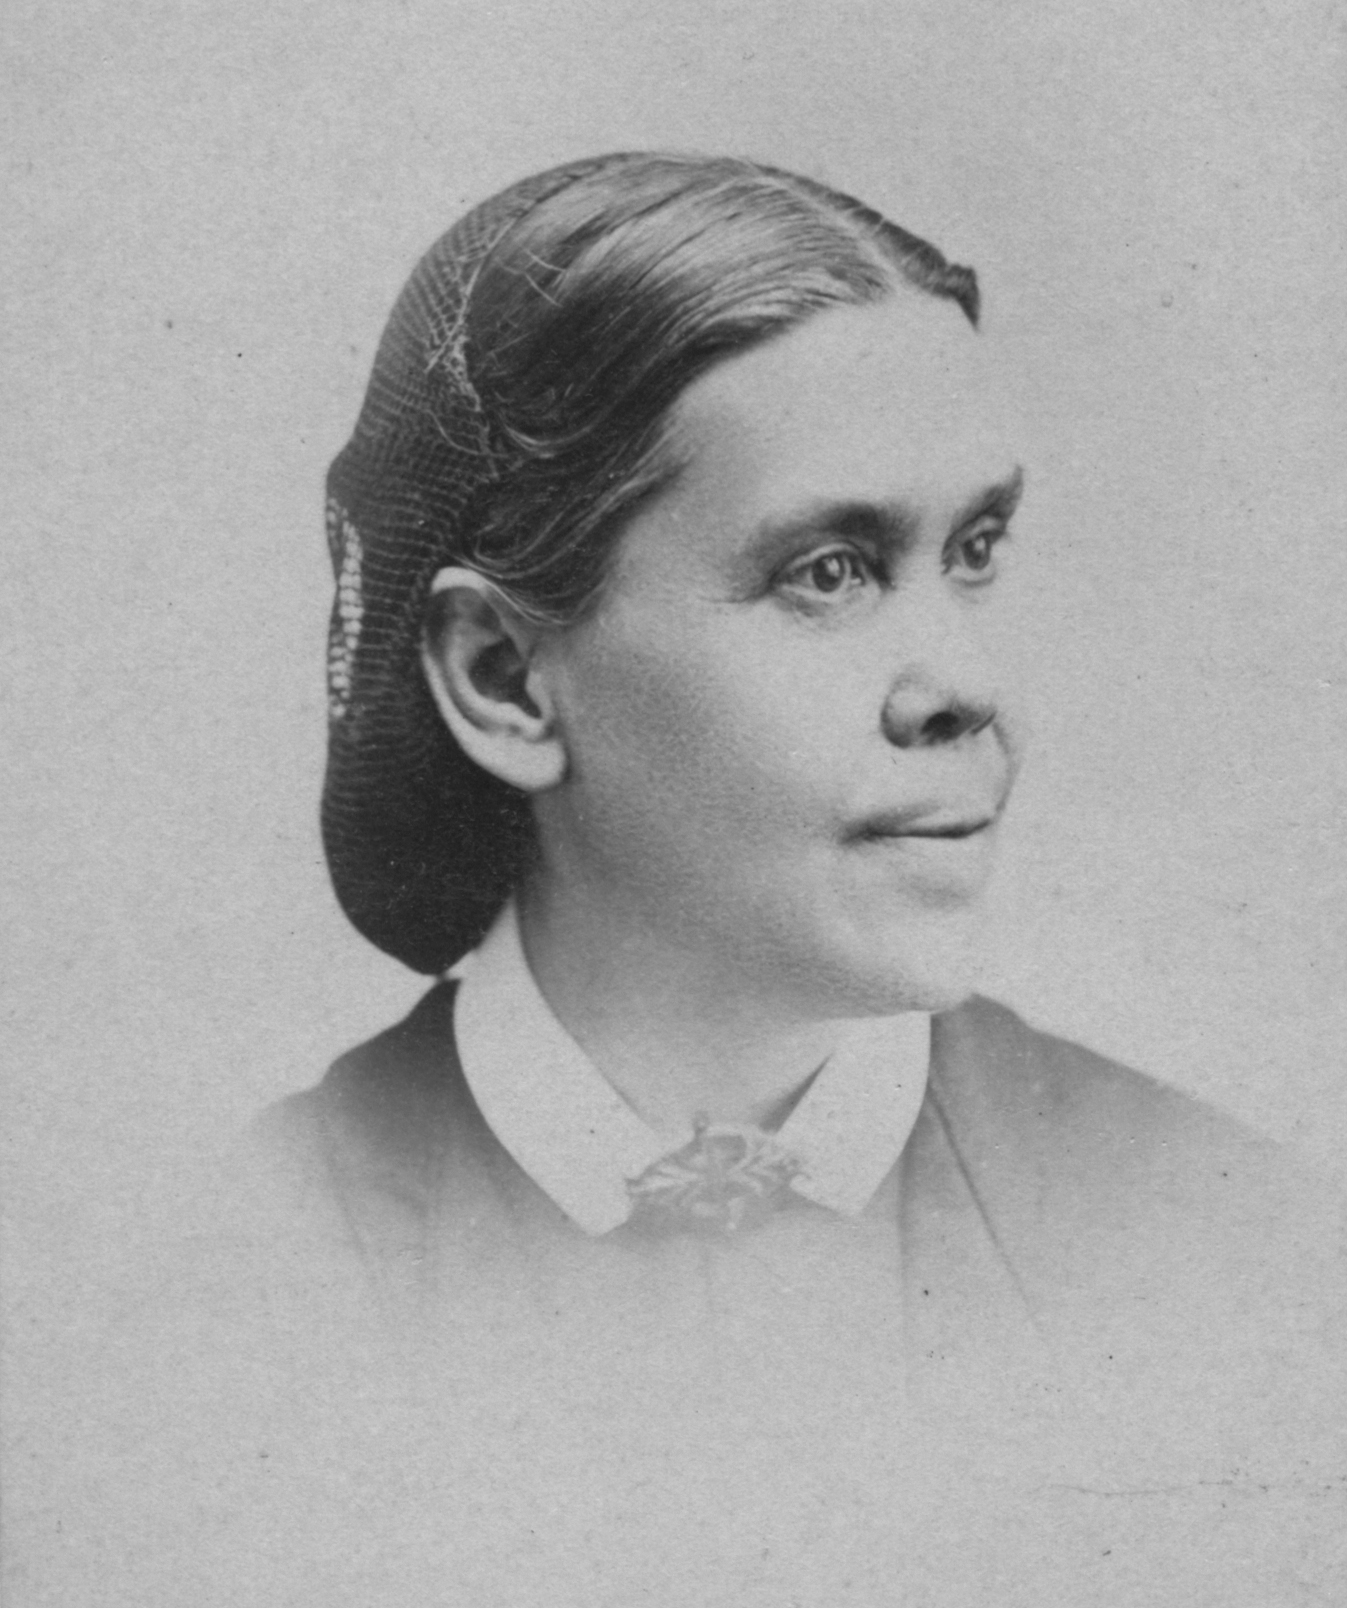
\includegraphics[width=0.65\linewidth]{images/ellen-white.jpg}
    \caption*{Ellen G. White}
    \label{fig:ellen-g-white}
\end{figure}


Consider the first point of the \emcap{Fundamental Principles}, which states that Seventh-day Adventists believe in \others{one God, \textbf{a personal, spiritual being}.}[First point of the Fundamental Principles][https://forgotten-pillar.s3.us-east-2.amazonaws.com/A+declaration+of+the+fundamental+principles+taught+and+practiced+by+the+Seventh-day+Adventists++.pdf] This makes it clear that the central issue in the doctrine of the \emcap{personality of God} concerns the outward, bodily form of the Father. But why was this such a vital and significant question? What were the implications of God having a bodily, personal form?


Considérez le premier point des \emcap{Principes Fondamentaux}, qui déclare que les Adventistes du Septième Jour croient en \others{un seul Dieu, \textbf{un être personnel et spirituel}.}[Premier point des Principes Fondamentaux][https://forgotten-pillar.s3.us-east-2.amazonaws.com/A+declaration+of+the+fundamental+principles+taught+and+practiced+by+the+Seventh-day+Adventists++.pdf] Cela montre clairement que la question centrale dans la doctrine de la \emcap{personnalité de Dieu} concerne la forme extérieure, corporelle du Père. Mais pourquoi était-ce une question si vitale et significative ? Quelles étaient les implications du fait que Dieu ait une forme corporelle et personnelle ?


\othersQuote{But because the pioneers of the Seventh-day Adventist Church held that prophecy was fulfilled on October 22, 1844, and that an important work began in heaven in the Most Holy Place of the heavenly sanctuary at that time, and because the Adventists who had become \textbf{spiritualizers} took the position that Christ had come into their hearts on October 22, 1844, and that His kingdom was in their hearts, the founders of the church, and notably Ellen White, were classed by the world generally, and also by those that SDAs have termed first-day Adventists, as one and the same group. Here again the great enemy cast aspersion upon the true, paralleling it with a false, spurious experience.}[ALW, 1BIO 80.2; 1985][https://egwwritings.org/read?panels=p668.587]


\othersQuote{Mais parce que les pionniers de l'Église Adventiste du Septième Jour soutenaient que la prophétie s'était accomplie le 22 octobre 1844, et qu'un travail important avait commencé dans le ciel dans le Lieu Très Saint du sanctuaire céleste à ce moment-là, et parce que les Adventistes qui étaient devenus \textbf{spiritualistes} avaient pris la position que Christ était entré dans leurs cœurs le 22 octobre 1844, et que Son royaume était dans leurs cœurs, les fondateurs de l'église, et notamment Ellen White, ont été classés par le monde en général, et aussi par ceux que les Adventistes du Septième Jour ont appelés adventistes du premier jour, comme un seul et même groupe. Ici encore, le grand ennemi a jeté l'opprobre sur le vrai, le mettant en parallèle avec une expérience fausse et falsifiée.}[ALW, 1BIO 80.2; 1985][https://egwwritings.org/read?panels=p668.587]


\othersQuoteNoGap{Ellen White was to speak of this matter again, particularly in the closing paragraphs of her first little book, Experience and Views, published in 1851. As one reads this he will note the use of \textbf{the term spiritualism}, which must be taken in the light of the work of the spiritualizers and not in the light of what today is understood to be spiritualism or spiritism, although both emanate from the same source.}[ALW, 1BIO 80.3; 1985][https://egwwritings.org/read?panels=p668.588]


\othersQuoteNoGap{Ellen White devait parler de cette question à nouveau, particulièrement dans les paragraphes de conclusion de son premier petit livre, Experience and Views, publié en 1851. En lisant cela, on remarquera l'utilisation de \textbf{le terme spiritualisme}, qui doit être compris à la lumière du travail des spiritualistes et non à la lumière de ce qu'on entend aujourd'hui par spiritualisme ou spiritisme, bien que les deux émanent de la même source.}[ALW, 1BIO 80.3; 1985][https://egwwritings.org/read?panels=p668.588]


\othersQuoteNoGap{We turn now to the statement written and published in 1851 as found in Ibid., 77, 78:}[ALW, 1BIO 80.4; 1985][https://egwwritings.org/read?panels=p668.589]


\othersQuoteNoGap{Nous nous tournons maintenant vers la déclaration écrite et publiée en 1851 comme on la trouve dans Ibid., 77, 78:}[ALW, 1BIO 80.4; 1985][https://egwwritings.org/read?panels=p668.589]


\othersQuoteNoGap{\textbf{I have frequently been falsely charged with teaching views peculiar to Spiritualism}. But before the editor of The Day-Star ran into that delusion, \textbf{the Lord \underline{gave me a view} of the sad and desolating effects that would be produced upon the flock by him and others \underline{in teaching the spiritual views}}.}[ALW, 1BIO 80.5; 1985][https://egwwritings.org/read?panels=p668.590]


\othersQuoteNoGap{\textbf{J'ai fréquemment été faussement accusée d'enseigner des vues propres au Spiritualisme}. Mais avant que l'éditeur de The Day-Star ne tombe dans cette illusion, \textbf{le Seigneur \underline{m'a donné une vision} des effets tristes et dévastateurs qui seraient produits sur le troupeau par lui et d'autres \underline{en enseignant les vues spiritualistes}}.}[ALW, 1BIO 80.5; 1985][https://egwwritings.org/read?panels=p668.590]


\othersQuoteNoGap{I have often seen the lovely \textbf{Jesus, that He is a person}. I asked Him \textbf{\underline{if His Father was a person} and \underline{had a form} like Himself}. Said Jesus, ‘I am in \textbf{the express image of My Father’s person}.}[ALW, 1BIO 80.6; 1985][https://egwwritings.org/read?panels=p668.591]


\othersQuoteNoGap{J'ai souvent vu le bien-aimé \textbf{Jésus, qu'Il est une personne}. Je Lui ai demandé \textbf{\underline{si Son Père était une personne} et \underline{avait une forme} comme Lui-même}. Jésus a dit: ‘Je suis \textbf{l'empreinte de sa personne}.}[ALW, 1BIO 80.6; 1985][https://egwwritings.org/read?panels=p668.591]


\othersQuoteNoGap{\textbf{I have often seen that \underline{the spiritual view} took away all the glory of heaven, and that in many minds the throne of David and the lovely person of Jesus have been burned up in the fire of Spiritualism.} I have seen that some who have been deceived and led into this error will be brought out into the light of truth, but it will be almost impossible for them to get entirely rid of \textbf{the deceptive power of Spiritualism}. Such should make thorough work in confessing their errors and leaving them forever.}[ALW, 1BIO 80.7; 1985][https://egwwritings.org/read?panels=p668.592]


\othersQuoteNoGap{\textbf{J'ai souvent vu que \underline{la vue spiritualiste} a enlevé toute la gloire du ciel, et que dans l'esprit de beaucoup, le trône de David et la personne bien-aimée de Jésus ont été consumés dans le feu du Spiritualisme.} J'ai vu que certains qui ont été trompés et conduits dans cette erreur seront amenés à la lumière de la vérité, mais il leur sera presque impossible de se débarrasser entièrement de \textbf{la puissance trompeuse du Spiritualisme}. Ces personnes devraient faire un travail approfondi en confessant leurs erreurs et en les abandonnant pour toujours.}[ALW, 1BIO 80.7; 1985][https://egwwritings.org/read?panels=p668.592]


\othersQuoteNoGap{\textbf{The spiritualization of heaven, God, Christ, and the coming of Christ lay at the foundation of much of the fanatical teachings that 17-year-old Ellen Harmon was called upon by God to meet in those formative days. The visions firmly established \underline{the personality of God and Christ}, \underline{the reality of heaven} and the reward to the faithful, and the resurrection. This sound guidance saved the emerging church}.}[ALW, 1BIO 81.1; 1985][https://egwwritings.org/read?panels=p668.595]


\othersQuoteNoGap{\textbf{La spiritualisation du ciel, de Dieu, du Christ et de la venue du Christ était à la base d'une grande partie des enseignements fanatiques que Ellen Harmon, âgée de 17 ans, fut appelée par Dieu à affronter en ces jours de formation. Les visions ont fermement établi \underline{la personnalité de Dieu et du Christ}, \underline{la réalité du ciel} et la récompense pour les fidèles, et la résurrection. Cette orientation saine a sauvé l'église naissante}.}[ALW, 1BIO 81.1; 1985][https://egwwritings.org/read?panels=p668.595]


The mistake of the Millerite movement in 1844 lay in misunderstanding the nature of the event, not its timing. Daniel 7:13-14 describes Christ coming to the Ancient of Days in heaven to receive dominion, glory, and a kingdom—not His second coming to earth. This event, marking the beginning of Christ’s work in the Most Holy Place, occurred at the conclusion of the 2300-day prophecy in 1844. Unlike other Adventist groups, the emerging Seventh-day Adventist Church uniquely recognized this heavenly event.


L'erreur du mouvement millérite en 1844 résidait dans la mauvaise compréhension de la nature de l'événement, et non de son timing. Daniel 7:13-14 décrit Christ venant vers l'Ancien des Jours dans le ciel pour recevoir la domination, la gloire et un royaume—pas Son second avènement sur terre. Cet événement, marquant le début de l'œuvre de Christ dans le Lieu Très Saint, s'est produit à la conclusion de la prophétie des 2300 jours en 1844. Contrairement aux autres groupes adventistes, l'Église Adventiste du Septième Jour naissante a reconnu de façon unique cet événement céleste.


This understanding is built on key premises:
\begin{itemize}
    \item Heaven is a real, literal place (John 14:1-3).
    \item There is a literal sanctuary in heaven where Christ ministers (Hebrews 8:2). 
    \item A real, physical throne exists in this sanctuary, occupied by God Himself (Daniel 7:9-10; Revelation 4:2-3; Ezekiel 1:26-28; Psalm 11:4).
\end{itemize}


Cette compréhension est fondée sur des prémisses clés:
\begin{itemize}
    \item Le ciel est un lieu réel et littéral (Jean 14:1-3).
    \item Il existe un sanctuaire littéral dans le ciel où Christ exerce son ministère (Hébreux 8:2). 
    \item Un trône réel et physique existe dans ce sanctuaire, occupé par Dieu Lui-même (Daniel 7:9-10; Apocalypse 4:2-3; Ézéchiel 1:26-28; Psaume 11:4).
\end{itemize}


Why is the question of the Father’s bodily form so important? If God were not a physical being, there would be no need for a literal throne, sanctuary, or heavenly ministry. A spiritualized interpretation undermines the foundation of Seventh-day Adventist theology, leading to a domino effect that erodes the doctrine of Christ’s priestly work.


Pourquoi la question de la forme corporelle du Père est-elle si importante? Si Dieu n'était pas un être physique, il n'y aurait pas besoin d'un trône littéral, d'un sanctuaire ou d'un ministère céleste. Une interprétation spiritualisée sape le fondement de la théologie adventiste du septième jour, conduisant à un effet domino qui érode la doctrine de l'œuvre sacerdotale du Christ.


The doctrine of the \emcap{personality of God} was a simple yet foundational teaching, affirmed in the first point of the \emcap{Fundamental Principles}: \textit{“One God, a personal, spiritual being.”} As such, He is not omnipresent by Himself but through His representative, the Holy Spirit.\footnote{The first point of the Fundamental Principles: \othersQuote{That there is \textbf{one God}, \textbf{a \underline{personal, spiritual being}}, the creator of all things, omnipotent, … and \textbf{everywhere present by \underline{his representative}, the Holy Spirit}. Ps. 139:7.}} When Ellen White asked Jesus \egwinline{if His Father \textbf{was a person} and \textbf{had a \underline{form}} like Himself,}[EW 77.1; 1882][https://egwwritings.org/read?panels=p28.490&index=0] we see clearly that the \textit{outward bodily \textbf{form}} is \textit{the quality or state} defining God as a person. This understanding was central in addressing the Kellogg crisis regarding \textit{The Living Temple}, which deviated from this core belief.


La doctrine de la \emcap{personnalité de Dieu} était un enseignement simple mais fondamental, affirmé dans le premier point des \emcap{Principes Fondamentaux} : \textit{“Un seul Dieu, un être personnel et spirituel.”} En tant que tel, Il n'est pas omniprésent par Lui-même mais par Son représentant, le Saint-Esprit.\footnote{Le premier point des Principes Fondamentaux : \othersQuote{Qu'il y a \textbf{un seul Dieu}, \textbf{un \underline{être personnel et spirituel}}, le créateur de toutes choses, omnipotent, … et \textbf{présent partout par \underline{son représentant}, le Saint-Esprit}. Ps. 139:7.}} Quand Ellen White a demandé à Jésus \egwinline{si Son Père \textbf{était une personne} et \textbf{avait une \underline{forme}} comme Lui-même,}[EW 77.1; 1882][https://egwwritings.org/read?panels=p28.490&index=0] nous voyons clairement que la \textit{forme \textbf{corporelle} extérieure} est \textit{la qualité ou l'état} qui définit Dieu comme une personne. Cette compréhension était centrale pour aborder la crise de Kellogg concernant \textit{Le Temple Vivant (le livre)}, qui s'écartait de cette croyance fondamentale.


But do our current \textit{Fundamental Beliefs} still affirm this doctrine? Do they explicitly teach that God is a real person with a bodily form, whose literal presence is in heaven, while He is omnipresent through His Spirit? The doctrine of God’s presence and personality is absent from today’s official beliefs. While individually, we may still believe in it, why was such a vital teaching omitted? What were the reasons behind this shift? These are the questions we must explore further in the context of \textit{The Foundation of Our Faith}.


Mais nos \textit{croyances fondamentales} actuelles affirment-elles toujours cette doctrine ? Enseignent-elles explicitement que Dieu est une personne réelle avec une forme corporelle, dont la présence littérale est au ciel, tandis qu'Il est omniprésent par Son Esprit ? La doctrine de la présence et de la personnalité de Dieu est absente des croyances officielles d'aujourd'hui. Bien qu'individuellement, nous puissions encore y croire, pourquoi un enseignement si vital a-t-il été omis ? Quelles étaient les raisons de ce changement ? Ce sont les questions que nous devons explorer davantage dans le contexte de \textit{La Fondation de Notre Foi}.


% The Historical Context

\begin{titledpoem}
    
    \stanza{
        By visions Ellen White stood firm, \\
        Against false views; she did affirm. \\
        The Father’s form, a truth profound, \\
        In this essential faith was found.
    }

    \stanza{
        "Spiritualizers" sought to claim \\
        That heaven’s realm was but a name. \\
        Yet God has form, like Christ His Son, \\
        This truth our founders built upon.
    }

    \stanza{
        A Spirit Person God does reign \\
        The universe is His domain \\
        This doctrine once our cornerstone, \\
        Has somehow from our statements flown.
    }
    
\end{titledpoem}